\chapter{Objetivos}
\label{cap:capitulo2}

\begin{flushright}
\begin{minipage}[]{10cm}
\emph{Dame seis horas para talar un árbol y pasaré las primeras cuatro afilando el hacha}\\
\end{minipage}\\

Abraham Licoln\\
\end{flushright}

\vspace{1cm}

Una vez establecido el marco contextual de este proyecto, se procederá a
presentar una descripción del problema a abordar, así como el proceso creativo e
intelectual que guiará el desarrollo del mismo, lo que incluirá los requisitos
del proyecto, la metodología empleada y el plan de trabajo detallado.

%Escribe aquí un párrafo explicando brevemente lo que vas a contar en este capítulo. En este capítulo lo ideal es explicar cuáles han sido los objetivos que te has fijado conseguir con tu trabajo, qué requisitos ha de respetar el resultado final, y cómo lo has llevado a cabo; esto es, cuál ha sido tu plan de trabajo.\\

\section{Descripción del problema}
\label{sec:descripcion}

Este proyecto surge como respuesta a la escasa investigación sobre los flujos de
datos empleados en conjunto con ROS2, ofreciendo a su vez un entorno propicio
para la creación sencilla de distintas aplicaciones robóticas basadas en dichos
flujos de datos, que pueden replicar de manera versátil y sencilla los
comportamientos reactivos de los robots, eludiendo la complejidad inherente de
este \textit{middleware} robótico y dando lugar, por tanto, a un nuevo entorno
de programación más simple.

Además, tiene como objetivo secundario cerrar la brecha educativa entre la
enseñanza secundaria y universitaria, expuesta en la Sección
\ref{sec:robotica_educativa}, en la que queda reflejado el salto que existe en
la educación en robótica entre la etapa secundaria y la universitaria, debido a
la complejidad del código y de las plataformas de desarrollo utilizadas.

%[TODO] hacer correccion de julio y pasar aspell.
%[TODO] añadir esto:
% Partes del capítulo 1 que detallan demasiado para ser movidas a este capítulo:

%%% [Párrafo sobre la complejidad de la arquitectura de ROS]
%La complejidad mencionada en la Sección \ref{sec:robotica_educativa} puede verse
%ilustrada en la Figura \ref{fig:ros}, en la que se muestra un esquema
%simplificado de la arquitectura de ambas versiones de este \textit{middleware}
%que puede resultar abrumadora para aquellos que se están iniciando en este
%ámbito, ya que se muestra la creciente complejidad adquirida al pasar de ROS,
%que ya era suficientemente complejo, a ROS2, en el que ahora existen distintas
%implementaciones de \textit{middleware} de comunicaciones, y otras capas como al
%de transporte, el sistema operativo y el \textit{hardware}.


%%% [Párrafo de la primerísima y antigua versión de la introducción, que fue
%   comentado para moverla a este capítulo debido a su explicación tan detallada]

%La educación en robótica se basa en la robótica de bajo coste, normalmente en
%placas como Arduino o similares, las cuales son ideales para este uso, y a su
%vez limitan la capacidad del robot en cuestión y el hardware que se puede usar y
%consecuentemente limitan la creatividad y el aprendizaje de los niños. Una vez
%se llega a un cierto nivel de conocimientos, el siguiente paso suele ser la
%programación de robots con ROS2, donde existe un gran escalon de aprendizaje.
%Este trabajo busca simplificar el desarrollo del software en ROS2 y así reducir
%dicho escalón, para hacer más fácil este desarrollo, dando la posibilidad de
%crear aplicaciones robóticas más complejas para robots más completos y que
%permanecen dentro de la categoría de robots de bajo coste y por tanto siguen
%siendo asequibles para instituciones como colegios o institutos.\\




%\section{Problemas de ROS en relación con el aprendizaje}
%\label{sec:miseccion} % etiqueta para luego referenciar esta sección

%ROS es el estándar en robótica para la programación de robots, pero tiene un
%problema y es el gran escalón de aprendizaje que existe cuando se pasa de una
%placa simple como arduino, a robots más complejos con máquinas integradas como
%las placas Raspberry Pi o un ordenador portátil directamente. Esto conlleva a una gran
%diferencia entre la robótica que se enseña en los colegios e institutos a la que
%se enseña en universidades, y es debido, precisamente a la complejidad de código
%y enseñanza de ROS, para los cuales, se requiere incluso de varias asignaturas.
%Por eso en este trabajo se pretende incorporar un paso intermedio en este gran
%escalón.
%
%La propia naturaleza de este \textit{middleware} robótico obliga a programar
%nodos que se ejecutan iterativamente en bucle, sin necesidad de generar una
%topología de red concreta para saber de donde vienen o a donde van los datos, lo
%que puede ser un poco complicado de entender a primera vista para los niños.\\
%
%Además de este problema, existe otro relacionado con la congestión de red: los
%nodos de ROS2 se comunican a través de DDS, un protocolo de comunicaciones que
%genera una gran cantidad de mensajes de \textit{Discovery}, lo que conlleva
%consecuentemente a la generación de congestión de la red, y dificulta de esta
%manera la programacion de aplicaciones multirobóticas, que son un posible
%siguiente paso en la enseñanza de la robotica, para entender las comunicaciones
%entre los distintos robots.\\
%
%Este trabajo prentende solucionar tanto el problema del escalón de aprendizaje,
%suponiendo un paso intermedio en la enseñanza de la robótica, y el problema de
%la congestión de red generala por DDS, suponiendo una posible solución a la
%misma.\\
%
%El problema de la congestión se soluciona usando otro protocolo llamado Zenoh,
%con mejores prestaciones que DDS, y la simplicidad del código de ROS2, se ha
%conseguido gracias al uso de un \textit{framework} llamado Zenoh-Flow, que
%funciona sobre el protocolo mencionado y el cual le da nombre. Este
%\textit{framework} está pensado para la programación de flujos de datos,, por lo
%que hay que definir primero un flujo de datos que luego seguiran los nodos,
%activando su iteración al momento de recibir un dato, generando de esta manera
%un flujo de datos que pasa de nodo a nodo, a diferencia de ROS.\\
%
%La implementación conjunta con ROS es posible gracias a que Zenoh-flow permite
%serializar los datos que se quieren enviar, y existe un bridge que los traduce
%de Zenoh a DDS para que los nodos de ROS2 entiendan dicha información. Es por
%este motivo, que si se serializan los mensajes de la misma manera que se hace
%internamente en ROS2, se pueden seguir utilizando nodos ya implementado en ROS2,
%como puede ser la navegación.\\



%Cuenta aquí el objetivo u objetivos generales y, a continuación, concrétalos mediante objetivos específicos.

\section{Requisitos}
\label{sec:requisitos}

Para solucionar los problemas descritos, este trabajo deberá cumplir los
siguientes requisitos:

\begin{enumerate}
    \item{Se utilizará \textit{GNU/Linux}, con la distribución
        \textit{Ubuntu 22.04 LTS} como sistema operativo en todos los
        \textit{hardwares}.}
    \item{El sistema deberá desarrollar alguna forma de programación de flujos
        de datos con ROS2.}
    \item{El entorno de programación debe brindar la posibilidad de funcionar en
        conjunto con nodos de ROS2, permitiendo la comunicación con los mismos
        mediante \textit{topics}.}
    \item{Los \textit{softwares} utilizados deben ser compatibles para funcionar
        correctamente en conjunto.}
    \item{Las aplicaciones demostrativas que se desarrollen deben ser fácilmente
        reproducibles y desplegables tanto en un entorno simulado como en un
        ambiente educativo real o de laboratorio.}
    \item{El desarrollo del \textit{software} debe ser lo suficientemente
        sencillo para poder ser llevado a cabo por alumnos preuniversitarios.}
    \item{El \textit{hardware} utilizado debe ser suficientemente económico para
        ser adquirido por organismos educativos.}
\end{enumerate}



\section{Competencias}
\label{sec:requisitos}

Las competencias generales que se cumplen con la realización de este trabajo de
fin de grado, según la guía docente de la asignatura son las siguientes:

\begin{enumerate}
    \item{\textit{CB2.} Que los estudiantes sepan aplicar sus conocimientos a su
        trabajo o vocación de una forma profesional y posean las competencias
        que suelen demostrarse por medio de la elaboración y defensa de
        argumentos y la resolución de problemas dentro de su área de estudio.}
        Esta competencia se cumple con la realización de la parte del
        \textit{software} de este trabajo, en la que se aplican distintos
        conocimientos adquiridos durante el grado.
    \item{\textit{CB4.} Que los estudiantes puedan transmitir información,
        ideas, problemas y soluciones a un público tanto especializado como no
        especializado.}
        Esta competencia se adquiere al detallar todo el complejo proceso
        consecuente a este trabajo de manera clara y comprensible en el presente
        documento.
    \item{\textit{CB5.} Que los estudiantes hayan desarrollado aquellas
        habilidades de aprendizaje necesarias para emprender estudios
        posteriores con un alto grado de autonomía.}
        Esta competencia queda cumplida al adquirir los conocimientos
        suficientes para el desarrollo de este trabajo de manera completamente
        autónoma, a base de distintas pruebas y consultas en distintas fuentes:
        publicaciones científicas, foros de desarrollo en la web, etc.
\end{enumerate}

La competencia específica \textit{CE28} de la asignatura detalla lo
siguiente:
Desarrollo de las capacidades adecuadas para realizar un ejercicio original
individual (o excepcionalmente colectivo), presentarlo y defenderlo ante un
tribunal universitario, consistente en un proyecto en el ámbito de las
tecnologías específicas del campo de la Robótica de naturaleza profesional en el
que se sinteticen e integren las competencias adquiridas en las enseñanzas.
Esta última competencia se cumple con la creación de este proyecto, memoria y
documentación, y su defensa ante un tribunal.

%Describe los requisitos que ha de cumplir tu trabajo.

\section{Metodología}
\label{sec:metodologia}

La metodología utilizada sigue pautas de investigación sobre el estado del arte
previo al trabajo, y posteriormente sobre el \textit{software} utilizado,
siempre evaluando de antemano la compatibilidad con el \textit{hardware}
disponible, así como realizando pruebas pertinentes sobre su correcto
funcionamiento en los distintos entornos, incluyendo la simulación y el
laboratorio.

En relación con el desarrollo del \textit{software} demostrativo se siguió un
ciclo de desarrollo \textit{software} iterativo, que consiste en la
planificación del \textit{software}, el desarrollo del mismo, su consecuente
revisión mediante pruebas y su corrección, todo ello de manera periódica,
generando en cada una de las iteraciones un resultado ejecutable mejor que el
anterior, hasta conseguir al final una versión completamente funcional, como se
ve reflejado en la Figura \ref{fig:desarrollo_iterativo}.
Este proceso de desarrollo puede verse alineado con los principios de mejora
continua del ciclo de desarrollo PDCA (\textit{Plan}, \textit{Do},
\textit{Check}, \textit{Act}).

\begin{figure} [h!]
  \begin{center}
    \includegraphics[width=10cm]{figs/desarrollo_iterativo}
  \end{center}
  \caption{Esquema del desarrollo software iterativo.}
  \label{fig:desarrollo_iterativo}
\end{figure}\

Este desarrollo implicó pruebas periódicas en simulación con el fin de
identificar errores y perfeccionar los valores de los parámetros, para
posteriormente evaluar su funcionamiento en un entorno real, concretamente en el
Laboratorio de Robótica del Aulario 3 de la Universidad Rey Juan Carlos.

%Qué paradigma de desarrollo software has seguido para alcanzar tus objetivos.

\section{Plan de trabajo}
\label{sec:plantrabajo}

El desarrollo del proyecto ha comprendido varias etapas, que incluyen la
investigación del \textit{software} a utilizar, la investigación del estado del
arte, la implementación de una arquitectura \textit{software} funcional en los
distintos entornos y el desarrollo del \textit{software} demostrativo o de
ejemplo, comprendiendo un periodo de tiempo superior a un año, comenzando en
febrero de 2023 y finalizando en junio de 2024.

\begin{enumerate}
    \item{\textit{Investigación del software a utilizar.} Periodo de febrero a
        mayo de 2023 durante las prácticas de empresa, en las que estuve
        aprendiendo el funcionamiento de \textit{softwares} como Zenoh,
        Zenoh-Flow, Zenoh-bridge-DDS, CycloneDDS, y acerca de las
        telecomunicaciones entre robots, 35 horas semanales durante 4 meses.}
    \item{\textit{Investigación del estado del arte.} Periodo de junio a agosto
        de 2023, en el que se investigó acerca de los trabajos previos
        relacionados, y sobre la viabilidad y compatibilidad del proyecto.}
    \item{\textit{Implementación de una arquitectura software funcional en
        simulación.} Periodo de junio a agosto de 2023, en el que se consiguió
        un correcto funcionamiento del \textit{software} en simulación.}
    \item{\textit{Desarrollo de software demostrativo.} Periodo de agosto a
        noviembre de 2023 en el que se migró el \textit{software} desarrollado
        durante las prácticas a versiones posteriores.}
    \item{\textit{Implementación de una arquitectura software funcional en un
        entorno real.} Periodo de noviembre de 2023 a enero de 2024 en el que se
        consiguió un correcto funcionamiento del \textit{software} en el
        laboratorio.}
    \item{\textit{Pruebas del software desarrollado en el laboratorio.} Periodo
        de noviembre de 2023 a abril de 2024 en el que se realizaron las pruebas
        y cambios necesarios para un correcto funcionamiento del
        \textit{software} demostrativo en el entorno real del laboratorio.}
    \item{\textit{Escritura de la memoria.} Periodo de mayo a junio de 2024 en el
        que se elaboró el presente documento, así como la presentación para su
        defensa.}
\end{enumerate}

Durante los periodos de desarrollo de este proyecto fuera de las prácticas de
empresa, se dedicaban aproximadamente de 30 a 40 horas semanales, manteniendo
reuniones con el tutor, que generalmente se llevaban a cabo semanalmente, y
ocasionalmente cada dos semanas.

Todo el proceso de trabajo se ha ido alojando en un repositorio público de
GitHub\footnote{https://github.com/RoboticsURJC/tfg-unai}.
Asimismo, el trabajo diario se ha ido documentando detalladamente en la
Wiki\footnote{https://github.com/RoboticsURJC/tfg-unai/wiki} de dicho
repositorio, haciendo las veces de cuaderno de bitácora, donde quedan reflejados
todos los contratiempos, soluciones y pruebas realizados.

%Qué agenda has seguido. Si has ido manteniendo reuniones semanales, cumplimentando objetivos parciales, si has ido afinando poco a poco un producto final completo, etc.
